
\documentclass[12pt,letterpaper]{article}

\usepackage[brazilian]{babel}
\usepackage[utf8]{inputenc}
\usepackage[T1]{fontenc}
\usepackage{fullpage}
\usepackage{cancel}
\usepackage{booktabs}
\usepackage[top=2cm, bottom=4.5cm, left=2.5cm, right=2.5cm]{geometry}
\usepackage{amsmath,amsthm,amsfonts,amssymb,amscd}
\usepackage{lastpage}
\usepackage{enumerate}
\usepackage{fancyhdr}
\usepackage{mathrsfs}
\usepackage{xcolor}
\usepackage{graphicx}
\usepackage{listings}
\usepackage{hyperref}
\usepackage[
backend=bibtex,
sorting=ynt
]{biblatex}
\addbibresource{refs.bib}

\newtheorem{defi}{Definição}
\newtheorem{teo}{Teorema}
\newtheorem{prop}{Propriedade}
\hypersetup{%
	colorlinks=true,
	linkcolor=blue,
	linkbordercolor={0 0 1}
}

\setlength{\parindent}{0.0in}
\setlength{\parskip}{0.05in}

\newcommand\course{Rener Oliveira}
\newcommand\lcur{\mathcal{L}}
\newcommand{\real}{\mathbb{R}}
\newcommand{\rr}{\mathbb{R}^2}
\newcommand{\rn}{\mathbb{R}^n}
\newcommand{\linesep}{{\color{black} \rule{\linewidth}{0.5mm} }}
\newcommand{\rpos}{\mathbb{R}_{>0}}
\newcommand{\blue}[1]{{\color{blue}{#1}}}
\newcommand{\bd}[1]{\boldsymbol{#1}}
\newcommand{\gt}{>}%broken keyboard
\newcommand{\pow}{^}%broken keyboard
\newcommand{\pr}{\operatorname{Pr}} %% probability
\newcommand{\vr}{\operatorname{Var}} %% variance
\newcommand{\rs}{X_1, X_2, \ldots, X_p} %%  random sample
\newcommand{\irs}{X_1, X_2, \ldots} %% infinite random sample
\newcommand{\rsd}{x_1, x_2, \ldots, x_p} %%  random sample, realised
\newcommand{\Sm}{\bar{X}_n} %%  sample mean, random variable
\newcommand{\sm}{\bar{x}_n} %%  sample mean, realised
\newcommand{\Sv}{\bar{S}^2_n} %%  sample variance, random variable
\newcommand{\sv}{\bar{s}^2_n} %%  sample variance, realised
\newcommand{\bX}{\boldsymbol{X}} %%  random sample, contracted form (bold)
\newcommand{\bx}{\boldsymbol{x}} %%  random sample, realised, contracted form (bold)
\newcommand{\bT}{\boldsymbol{T}} %%  Statistic, vector form (bold)
\newcommand{\bt}{\boldsymbol{t}} %%  Statistic, realised, vector form (bold)
\newcommand{\emv}{\hat{\theta}_{\text{EMV}}}
\newcommand{\defn}{\stackrel{\textrm{\scriptsize def}}{=}}
\newcommand{\op}{\operatorname}
\newcommand{\eps}{\varepsilon}
\newcommand{\norm}{\mathcal{N}}
\newcommand{\iid}{\overset{\text{iid}}{\sim}}
\pagestyle{fancyplain}
\headheight 35pt        
\chead{\textbf{\Large Regressão \\Linear Bayesiana}}
\lhead{Modelagem Estatística\\Trabalho A1}
\rhead{\small{\course \\ \today}}
\lfoot{}
\cfoot{}
\rfoot{\small\thepage}
\headsep 1.5em
\usepackage{xcolor}
\definecolor{maroon}{cmyk}{0, 0.87, 0.68, 0.32}
\definecolor{halfgray}{gray}{0.55}
\definecolor{ipython_frame}{RGB}{207, 207, 207}
\definecolor{ipython_bg}{RGB}{247, 247, 247}
\definecolor{ipython_red}{RGB}{186, 33, 33}
\definecolor{ipython_green}{RGB}{0, 128, 0}
\definecolor{ipython_cyan}{RGB}{64, 128, 128}
\definecolor{ipython_purple}{RGB}{170, 34, 255}

\usepackage{listings}
\lstset{
	breaklines=true,
	%
	extendedchars=true,
	literate=
	{á}{{\'a}}1 {é}{{\'e}}1 {í}{{\'i}}1 {ó}{{\'o}}1 {ú}{{\'u}}1
	{Á}{{\'A}}1 {É}{{\'E}}1 {Í}{{\'I}}1 {Ó}{{\'O}}1 {Ú}{{\'U}}1
	{à}{{\`a}}1 {è}{{\`e}}1 {ì}{{\`i}}1 {ò}{{\`o}}1 {ù}{{\`u}}1
	{À}{{\`A}}1 {È}{{\'E}}1 {Ì}{{\`I}}1 {Ò}{{\`O}}1 {Ù}{{\`U}}1
	{ä}{{\"a}}1 {ë}{{\"e}}1 {ï}{{\"i}}1 {ö}{{\"o}}1 {ü}{{\"u}}1
	{Ä}{{\"A}}1 {Ë}{{\"E}}1 {Ï}{{\"I}}1 {Ö}{{\"O}}1 {Ü}{{\"U}}1
	{â}{{\^a}}1 {ê}{{\^e}}1 {î}{{\^i}}1 {ô}{{\^o}}1 {û}{{\^u}}1
	{Â}{{\^A}}1 {Ê}{{\^E}}1 {Î}{{\^I}}1 {Ô}{{\^O}}1 {Û}{{\^U}}1
	{œ}{{\oe}}1 {Œ}{{\OE}}1 {æ}{{\ae}}1 {Æ}{{\AE}}1 {ß}{{\ss}}1
	{ç}{{\c c}}1 {Ç}{{\c C}}1 {ø}{{\o}}1 {å}{{\r a}}1 {Å}{{\r A}}1
	{€}{{\EUR}}1 {£}{{\pounds}}1
}

%%
%% Python definition (c) 1998 Michael Weber
%% Additional definitions (2013) Alexis Dimitriadis
%% modified by me (should not have empty lines)
%%
\lstdefinelanguage{iPython}{
	morekeywords={access,and,break,class,continue,def,del,elif,else,except,exec,finally,for,from,global,if,import,in,is,lambda,not,or,pass,print,raise,return,try,while},%
	%
	% Built-ins
	morekeywords=[2]{abs,all,any,basestring,bin,bool,bytearray,callable,chr,classmethod,cmp,compile,complex,delattr,dict,dir,divmod,enumerate,eval,execfile,file,filter,float,format,frozenset,getattr,globals,hasattr,hash,help,hex,id,input,int,isinstance,issubclass,iter,len,list,locals,long,map,max,memoryview,min,next,object,oct,open,ord,pow,property,range,raw_input,reduce,reload,repr,reversed,round,set,setattr,slice,sorted,staticmethod,str,sum,super,tuple,type,unichr,unicode,vars,xrange,zip,apply,buffer,coerce,intern},%
	%
	sensitive=true,%
	morecomment=[l]\#,%
	morestring=[b]',%
	morestring=[b]",%
	%
	morestring=[s]{'''}{'''},% used for documentation text (mulitiline strings)
	morestring=[s]{"""}{"""},% added by Philipp Matthias Hahn
	%
	morestring=[s]{r'}{'},% `raw' strings
	morestring=[s]{r"}{"},%
	morestring=[s]{r'''}{'''},%
	morestring=[s]{r"""}{"""},%
	morestring=[s]{u'}{'},% unicode strings
	morestring=[s]{u"}{"},%
	morestring=[s]{u'''}{'''},%
	morestring=[s]{u"""}{"""},%
	%
	% {replace}{replacement}{lenght of replace}
	% *{-}{-}{1} will not replace in comments and so on
	literate=
	{á}{{\'a}}1 {é}{{\'e}}1 {í}{{\'i}}1 {ó}{{\'o}}1 {ú}{{\'u}}1
	{Á}{{\'A}}1 {É}{{\'E}}1 {Í}{{\'I}}1 {Ó}{{\'O}}1 {Ú}{{\'U}}1
	{à}{{\`a}}1 {è}{{\`e}}1 {ì}{{\`i}}1 {ò}{{\`o}}1 {ù}{{\`u}}1
	{À}{{\`A}}1 {È}{{\'E}}1 {Ì}{{\`I}}1 {Ò}{{\`O}}1 {Ù}{{\`U}}1
	{ä}{{\"a}}1 {ë}{{\"e}}1 {ï}{{\"i}}1 {ö}{{\"o}}1 {ü}{{\"u}}1
	{Ä}{{\"A}}1 {Ë}{{\"E}}1 {Ï}{{\"I}}1 {Ö}{{\"O}}1 {Ü}{{\"U}}1
	{â}{{\^a}}1 {ê}{{\^e}}1 {î}{{\^i}}1 {ô}{{\^o}}1 {û}{{\^u}}1
	{Â}{{\^A}}1 {Ê}{{\^E}}1 {Î}{{\^I}}1 {Ô}{{\^O}}1 {Û}{{\^U}}1
	{œ}{{\oe}}1 {Œ}{{\OE}}1 {æ}{{\ae}}1 {Æ}{{\AE}}1 {ß}{{\ss}}1
	{ç}{{\c c}}1 {Ç}{{\c C}}1 {ø}{{\o}}1 {å}{{\r a}}1 {Å}{{\r A}}1
	{€}{{\EUR}}1 {£}{{\pounds}}1
	%
	{^}{{{\color{ipython_purple}\^{}}}}1
	{=}{{{\color{ipython_purple}=}}}1
	%
	{+}{{{\color{ipython_purple}+}}}1
	{*}{{{\color{ipython_purple}$^\ast$}}}1
	{/}{{{\color{ipython_purple}/}}}1
	%
	{+=}{{{+=}}}1
	{-=}{{{-=}}}1
	{*=}{{{$^\ast$=}}}1
	{/=}{{{/=}}}1,
	literate=
	*{-}{{{\color{ipython_purple}-}}}1
	{?}{{{\color{ipython_purple}?}}}1,
	%
	identifierstyle=\color{black}\ttfamily,
	commentstyle=\color{ipython_cyan}\ttfamily,
	stringstyle=\color{ipython_red}\ttfamily,
	keepspaces=true,
	showspaces=false,
	showstringspaces=false,
	%
	rulecolor=\color{ipython_frame},
	frame=single,
	frameround={t}{t}{t}{t},
	framexleftmargin=6mm,
	numbers=left,
	numberstyle=\tiny\color{halfgray},
	%
	%
	backgroundcolor=\color{ipython_bg},
	%   extendedchars=true,
	basicstyle=\scriptsize,
	keywordstyle=\color{ipython_green}\ttfamily,
}
\begin{document}
	\tableofcontents
	\newpage
	\section{Introdução}
	
	A regressão linear é um modelo muito utilizado em diversas áreas de aplicações. Meu intuito com este trabalho era estudar a regressão linear sobre o ponto de vista bayesiano. Inicio com uma reapresentação dos métodos de estimação de coeficientes frequentista. 
	
	A inspiração surgiu na leitura de um texto do blog do PyMC3\cite{pymc3_glm}, biblioteca Python de análise bayesiana. O texto era um simples tutorial de como usar as ferramentas da biblioteca para fazer um regressão linear bayesiana simples (1 preditor) posterioris dos coeficientes via MCMC. O texto entretanto não justifica com clareza a escolha das formas funcionais das prioris. Decidi então buscar materiais mais teóricos sobre o assunto, e encontrei um capítulo de um livro\cite{o1994kendall}, que estebejecia resultados de uma análise conjugada dos parâmetros.
	
	Na seção seguinte após a revisão do método frequentista, inicio a discussão sobre regressão bayesiana, estabalecendo de forma simplificada os resultados de \cite{o1994kendall}. O produto final dessa seção teórica são fórmulas analíticas para parâmetros da distribuição à posteriori, partindo de um priori conjugada.
	
Depois disso faço uma simulação computacional similar à de \cite{pymc3_glm}, porém em maior dimensão, já que os resultados teóricos formalizados permitem esse tipo de extensão. São gerados dados sintéticos com parâmetros fixos para avaliar a qualidade das estimativa.
	
	Com a análise conjudada realizada, fiz uma implementação que gerava distribuições à posteriori amostrando das distribuições conjugadas obtidas analiticamente. E no final utilizei o MCMC para amostrar posterioris via Cadeia de Markov, utilizando as ferramentas da biblioteca PyMC3.
	
	Um trabalho futuro seria aplicar esses algoritmos em dados reais, porém neste texto me contentei com dados sintéticos, pois o intuito era apenas estudar a teoria bayesiana de regressões, e melhorar as implementações do blog\cite{pymc3_glm}.
	
	Durante o corpo do texto, deixo explícito alguns trechos de códigos python utilizado, porém todo o desenvolvimento computacional deste trabalho pode ser consultado \href{https://colab.research.google.com/drive/1fTrA95E2J-WBqXYz_lYunWlpAoco9IBI?usp=sharing}{neste link} do Google Colab, uma plataforma online de notebooks Jupyter.
	\newpage
	\section{O Modelo Frequentista}
	
	A regressão linear é um modelo que visa explicar a relação entre uma variável reposta real $\bd y$ e outras variáveis explicativas $\rs$ através de algumas premissas. No caso cada $X_j$ é um vetor coluna de $n$ observações $X_j = [x_{1j},x_{2j},\ldots,x_{nj}]^T$, assim como a variável resposta: $\bd y=[y_1,y_2,\ldots,y_n]^T$.
	
	A principal é a linearidade da esperança de $\bd y$ em relação aos predidores, isto é, existem $\beta_0,\beta_1,\ldots,\beta_p$ tais que 
	$$E[\bd y|\bd X]=\beta_0+\beta_1X_1+\ldots+\beta_pX_p$$
	
	Onde $\bd X$ é uma matrix $n\times(p+1)$, com $n$ sendo a quantidade de observações e $p$ a quantidade de preditores. O número de colunas p+1, se dá por conta da inclusão de uma coluna constante igual a 1, para que possamos representar a expressão acima de forma matricial (\textit{design matrix}).
	$$\bd X=
	\begin{bmatrix}
		1 & \vdots & \vdots & \ldots &\vdots\\
		\vdots & X_1 & X_2 & \ldots & X_n\\
		1 &\vdots & \vdots & \ldots &\vdots
	\end{bmatrix}$$

	Sendo $\beta=[\beta_0,\beta_1,\ldots,\beta_p]^T$ vetor coluna $(p+1)\times 1$, temos que:
	$$E[\bd y|\bd X]=\bd X\beta$$
	
	Um outra hipótese importante é a de normalidade, ou seja,
	$$\bd y=\bd X\beta+\varepsilon,$$
	
	onde o vetor de ruídos $\varepsilon=[\varepsilon_1,\varepsilon_2,\ldots,\varepsilon_n]^T$ com cada $\eps_i\iid \norm(0,\sigma^2)$ .
	
	Disso segue a hipótese de homocedasticidade, ou seja, variância comum entre as observações.
	
	No modelo linear frequentista, se assume que os coeficientes $\beta$ são valores fixos. Assim, a estimação ocorre por minimização dos erros quadráticos, ou seja, o estimador $\hat\beta=[\hat\beta_0,\hat\beta_1,\ldots,\hat\beta_p]^T$ é tal que minimiza a forma quadrática de perda:
	$$RSS = (\bd y-\bd X \beta)^T(\bd y-\bd X\beta),$$
	
	onde $RSS$ é uma sigla em inglês para soma dos resíduos ao quadrado (\textit{residual sum of squares}).
	
	Segundo \cite{degroot2012probability} o vetor que minimiza o erro acima é dados por:
	\begin{align}\hat\beta=(\bd X^T\bd X)^{-1}\bd X^T\bd y\label{betafreq}\end{align}
	
\section{O Modelo Bayesiano}
	
	No paradigma bayesiano, os coeficientes $\beta_i$, com $i=0,1,\ldots,p$ deixam de ser considerados como valores fixos e passam a ser variáveis aleatórias. A hipótese de normalidade (iid) se mantém, ou seja, se $\bd x_i$ é a i-ésima linha da matrix $\bd X$. 
	
	\begin{align}y_i|\bd x_i,\beta,\sigma^2\iid\norm(\bd x_i\beta,\sigma^2)\label{lik}
	\end{align}
	
	Nesta seção vamos mostrar os passos da derivação de uma família de distribuições à priori conjugadas para $\sigma^2$ e para $\beta|\sigma^2$. O objetivo será obter uma forma funcional para distribuição à posteriori conjunta dos parâmetros desconhecidos $p(\beta,\sigma^2|\bd X,\bd y)$.
	Desta forma é possível gerar distribuições para novos dados y não previamente observados, ao invés de um valor fixo, como no caso frequentista.
	
	A verossimilhança condicional $p(\bd y|\bd X,\beta,\sigma^2)$, pela distribuição por (\ref{lik}) será o produtório:
	\begin{align*}
		p(\bd y|\bd X,\beta,\sigma^2)&=\prod_{i=1}^{n}p(y_i|\bd x_i,\beta,\sigma^2)\\
		&\propto \prod_{i=1}^{n}(\sigma^2)^{-1/2}\exp\left(-\dfrac{1}{2\sigma^2}(y_i-\bd x_i\beta)^2\right)\\
		&=(\sigma^2)^{-n/2}\exp\left(-\dfrac{1}{2\sigma^2}\sum_i^n(y_i-\bd x_i\beta)^2\right)\\
		&=(\sigma^2)^{-n/2}\exp\left(-\dfrac{1}{2\sigma^2}(\bd y-\bd X\beta)^T(\bd y-\bd X\beta)\right)\\
	\end{align*}
	Podemos expandir a forma quadrática da exponencial, considerando $\hat\beta$ como o estimador frequentista dos coeficientes dado pela expressão (\ref{betafreq}).
	\begin{align*}(\bd y-\bd X\beta)^T(\bd y-\bd X\beta)&=\bd (\bd y^T-\beta^T\bd X^T)(\bd y-\bd X\beta)\\
		&=\bd y^T\bd y-\bd y^T\bd X\beta-\beta^T\bd X^T\bd y+\beta^T\bd X^T\bd X\beta\\
		&\text{ Completando o quadrado $\beta^T\bd X^T\bd X\beta$:}\\
		&=(\beta-\hat\beta)^T(\bd X^T\bd X)(\beta-\hat\beta)+\beta^T\bd X^T\bd X\hat\beta+\hat\beta^T\bd X^T\bd X\beta-\hat\beta^T\bd X^T\bd X\hat\beta\\
		&~~~~+\bd y^T\bd y-\bd y^T\bd X\beta-\beta^T\bd X\bd y\\
		&\text{Com alguns passos de Álgebra Linear usando a fórmula \ref{betafreq}, chegamos em:}\\
		&\hat\beta^T=\bd y^T\bd X(\bd X^T\bd X)^{-1}\end{align*}
		Substituindo na expressão acima, e fazendo mais algumas simplificações, chegamos em:
		$$(\bd y-\bd X\beta)^T(\bd y-\bd X\beta)=(\bd y-\bd X\hat\beta)^T(\bd y-\bd X\hat\beta)+(\beta-\hat\beta)^T(\bd X^T\bd X)(\beta-\hat\beta),$$ 
	Sendo assim, podemos fatorizar a verossimilhança de uma forma conveniente como abaixo:
	\begin{align}
		p(\bd y|\bd X,\beta,\sigma^2)&\propto (\sigma^2)^{-v/2}\exp\left(-\dfrac{vs^2}{2\sigma^2}\right)(\sigma^2)^{-\frac{n-v}{2}}\exp\left(-\dfrac{1}{2\sigma^2}(\beta-\hat\beta)^T(\bd X^T\bd X)(\beta-\hat\beta)\right),\label{lik2}
	\end{align}
	
	com $vs^2=(\bd y-\bd X\hat\beta)^T(\bd y-\bd X\hat\beta)$ e $v=n-(p+1)$.
	
	A forma funcional acima é a multiplicação do núcleo da densidade de uma Gama Inversa com o núcleo de uma Normal. Isso sugere a elicitação de prioris dessas distribuições para $p(\beta,\sigma^2)=p(\sigma^2)p(\beta|\sigma^2)$. 
	
	As prioris conjugadas serão então:
	\begin{align}
		\sigma^2& \sim\op{Inv-Gamma}(a_0,b_0)\label{priors2}\\
		\beta|\sigma^2&\sim \norm(\bd\mu_0,\sigma^2\bd\Lambda_0^{-1})\label{priorbs},
	\end{align}
	
	onde $a_0=\dfrac{v_0}{2}$, $b_0=\dfrac{v_0s_0^2}{2}$, $\bd \mu_0$ é a média à priori para $\beta$ e $\bd\Lambda_0$ é uma matriz diagonal de precisão à priori. Nesse caso $v_0$ e $s_0^2$ podem ser interpretados como valores à priori para os graus de liberdade e para a variancia amostral, dado que a média da Gama Inversa é $\dfrac{b_0}{a_0-1}=\dfrac{v_0s_0^2}{v_0-2}$. A matriz de precisão é interpretada como o quão certo o modelador está em relação à sua priori $\bd\mu_0$.
	
	As densidades serão:
	\begin{align*}
		p(\sigma^2)&\propto(\sigma^2)^{-\frac{v_0}2-1}\exp\left(-\dfrac{v_0s_0^2}{2\sigma^2}\right)\\
		p(\beta|\sigma^2)&\propto(\sigma^2)^{-\frac{p+1}{2}}\exp\left(-\dfrac{1}{2\sigma^2}(\beta-\bd\mu_0)^T\bd\Lambda_0(\beta-\bd\mu_0)\right)
	\end{align*}

	Unindo as prioris acima com a verossimilhança em (\ref{lik2}) e fazendo uma reorganização dos termos que será omitida aqui, é possível chegar em:
	\begin{align*}
		p(\beta,\sigma^2|\bd y,\bd X)&\propto p(\bd y|\bd X,\beta,\sigma^2)p(\beta|\sigma^2)p(\sigma^2)\\
		&\propto(\sigma^2)^{-\frac{p+1}{2}}\exp\left(-\dfrac{1}{2\sigma^2}(\beta-\bd\mu_n)^T(\bd X^T\bd X+\bd\Lambda_0)(\beta-\bd\mu_n)\right)\\
		&\times(\sigma^2)^{-\frac{n+2a_0}{2}-1}\exp\left(-\dfrac{2b_0\bd y^T\bd y-\bd \mu_n^T(\bd X^T\bd X+\bd\Lambda_0)\bd\mu_ n+\bd\mu_0^T\bd\lambda_0\bd\mu_0}{2\sigma^2}\right),
	\end{align*}

	com $\bd\mu_n=(\bd X^T\bd X+\bd\Lambda_0)^{-1}(\bd X^T\bd X\hat\beta+\bd\Lambda\bd\mu_0)$.
	
	A posteriori pode ser escrita então como o produto das posterioris de $\beta|\sigma^2$ e de $\sigma^2$, onde
	\begin{align*}\sigma^2|\bd y,\bd X&\sim \op{Inv-Gamma}(a_n,b_n)\\
		\beta|\sigma^2,\bd y,\bd X &\sim \norm(\bd\mu_n,\sigma^2\bd\Lambda_n^{-1}),		
	\end{align*}
	
	na qual os novos parâmetros são:
	\begin{align}
		\bd\mu_n&=(\bd X^T\bd X+\bd\Lambda_0)^{-1}(\bd X^T\bd X\hat\beta+\bd\Lambda_ 0\bd\mu_0)\nonumber\\
		\bd\Lambda_n&=\bd X^T \bd X+\bd\Lambda_0\nonumber\\
		a_n&=a_0+\dfrac{n}{2}\label{posteriorformulas}\\
		b_n&=b_0+\dfrac{\bd y^T\bd y-\bd \mu_n^T\bd\Lambda_n\bd\mu_ n+\bd\mu_0^T\bd\Lambda_0\bd\mu_0}{2}\nonumber
	\end{align}
	
	De fato, tal distribuição conjunta de $(\beta,\sigma^2)$ recebe o nome de $\op{Normal-Gamma-Inversa}$, e é uma família conjugada, como demonstrado com mais detalhes em \cite{o1994kendall}.
	
	\section{Simulações Computacionais}
	
	\subsection{Geração de dados}
	Nesta seção vamos gerar distribuições à posteriori para $(\beta,\sigma^2)$ de forma numérica utilizando MCMC e o amostrador NUTS, implementado no pacote PyMC3 da liguagem Python.
	
	A referência \cite{pymc3_glm}, do próprio site da biblioteca PyMC3, para exemplificar suas funcionalidades de modelos lineares bayesianos, faz uma simulação utilizando dados sintéticos normalmente distribuídos, porém é utilizada uma formulação com apenas um preditor, e uma distribuição diferente da que derivamos anteriormente para $p(\sigma^2)$. Vamos reproduzir o exemplo do site utilizando dados gerados sinteticamente a partir da seguinte lei:
	\begin{align*}Y=\beta_0+\beta_1X_1+\beta_2X_2+\eps\\
		\eps\sim\norm\left(0,\sigma^2\bd I\right)\end{align*}
	
	Com variância $\sigma^2=4$, vetor de coeficientes escolhido como $\beta = [-1,3,6]^T$. Além disso, usamos $n=350$ pontos de dados.
	
	No caso, $X_1$ é um vetor de $n$ pontos igualmente espaçados em $[0,1]$ e $X_2$ é gerado à de uma distribuição uniforme em $[0,1]$.
	
	Na Figura \ref{data1} foi plotado um plano laranja que é a equação puramente linear, e 350 pontos azuis baseando-se na adição do erro $\eps$ aos pontos $\bd X\beta$
	
	\begin{figure}[!htb]
		\centering
		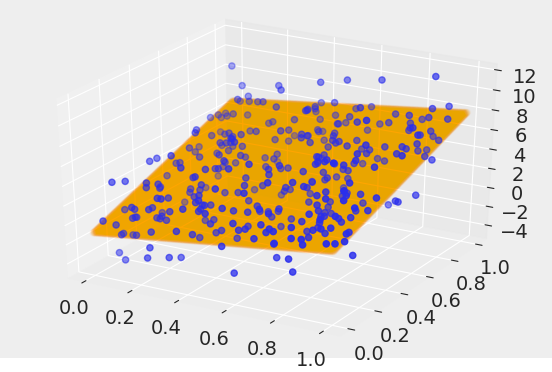
\includegraphics[scale=0.71]{../images/generated_data.png}
		\caption{Laranja: Plano base de geração dos pontos; Azul: Plano + $\eps$}
		\label{data1}
	\end{figure}

Abaixo segue o código de geração dos dados.

	\begin{lstlisting}[language=iPython]
n = 350

true_beta = [-1,3,6]
true_sigma2 = 2**2
X1 = np.linspace(0,1,n)
X2 = np.random.uniform(size = n)

# y = beta0+beta1*x1+beta2*x2
true_regression_plane = true_beta[0] + true_beta[1] * X1 + true_beta[2]*X2

# Adding Noise with variance true_sigma2
y = true_regression_plane + np.random.normal(scale=true_sigma2**(1/2), size=n)
	\end{lstlisting}
	
	\subsection{Estimação Frequentista}
 Utilizando o pacote statsmodels, podemos estimar uma regressão linear frequentista, nos dando estimadores pontuais para os coeficientes obtidos por minimização quadrática, ou equivalentemente neste caso, maximização da merossimilhança.
 
 Segue abaixo o relatório da regressão:
 
%	\begin{center}
%		\begin{tabular}{lclc}
%			\toprule
%			\textbf{Dep. Variable:}    &        y         & \textbf{  R-squared:         } &     0.493   \\
%			\textbf{Model:}            &       OLS        & \textbf{  Adj. R-squared:    } &     0.490   \\
%			\textbf{Method:}           &  Least Squares   & \textbf{  F-statistic:       } &     168.7   \\
%			\textbf{Date:}             & Tue, 13 Apr 2021 & \textbf{  Prob (F-statistic):} &  6.55e-52   \\
%			\textbf{Time:}             &     02:15:52     & \textbf{  Log-Likelihood:    } &   -734.69   \\
%			\textbf{No. Observations:} &         350      & \textbf{  AIC:               } &     1475.   \\
%			\textbf{Df Residuals:}     &         347      & \textbf{  BIC:               } &     1487.   \\
%			\textbf{Df Model:}         &           2      & \textbf{                     } &             \\
%			\bottomrule
%		\end{tabular}
%		\begin{tabular}{lcccccc}
%			& \textbf{coef} & \textbf{std err} & \textbf{t} & \textbf{P$> |$t$|$} & \textbf{[0.025} & \textbf{0.975]}  \\
%			\midrule
%			\textbf{const} &      -0.8526  &        0.278     &    -3.064  &         0.002        &       -1.400    &       -0.305     \\
%			\textbf{x1}    &       2.5465  &        0.366     &     6.955  &         0.000        &        1.826    &        3.267     \\
%			\textbf{x2}    &       6.0870  &        0.355     &    17.131  &         0.000        &        5.388    &        6.786     \\
%			\bottomrule
%		\end{tabular}
		%\caption{OLS Regression Results}
%	\end{center}
\begin{center}
	\begin{tabular}{lclc}
		\toprule
		\textbf{Dep. Variable:}    &        y         & \textbf{  R-squared:         } &     0.496   \\
		\textbf{Model:}            &       OLS        & \textbf{  Adj. R-squared:    } &     0.493   \\
		\textbf{Method:}           &  Least Squares   & \textbf{  F-statistic:       } &     170.7   \\
		\textbf{Date:}             & Tue, 13 Apr 2021 & \textbf{  Prob (F-statistic):} &  2.38e-52   \\
		\textbf{Time:}             &     21:08:53     & \textbf{  Log-Likelihood:    } &   -739.93   \\
		\textbf{No. Observations:} &         350      & \textbf{  AIC:               } &     1486.   \\
		\textbf{Df Residuals:}     &         347      & \textbf{  BIC:               } &     1497.   \\
		\textbf{Df Model:}         &           2      & \textbf{                     } &             \\
		\bottomrule
	\end{tabular}
	\begin{tabular}{lcccccc}
		& \textbf{coef} & \textbf{std err} & \textbf{t} & \textbf{P$> |$t$|$} & \textbf{[0.025} & \textbf{0.975]}  \\
		\midrule
		\textbf{const} &      -1.2781  &        0.288     &    -4.434  &         0.000        &       -1.845    &       -0.711     \\
		\textbf{x1}    &       2.5910  &        0.372     &     6.963  &         0.000        &        1.859    &        3.323     \\
		\textbf{x2}    &       6.4928  &        0.372     &    17.453  &         0.000        &        5.761    &        7.225     \\
		\bottomrule
	\end{tabular}
\end{center}

	Como os dados foram gerados de forma sintética obedecendo as principais premissas de Regressão Linear, obtivemos um resultado satisfatório com a estimação via OLS\footnote{Ordinary Least Squares}. A estimação foi $\hat\beta = [-1.2781,2.5910,6.4928]^T$ razoavelmente próximo do verdadeiro $\beta$. Perceba que os testes de hipótese $\op{Student-t}$ apontam estimadores estatisticamente significantes, O teste $F$ também deu um bom resultado. Além disso os intervalos de confiança $95\%$ cobrem os valores reais dos parâmetros; O comprimento de tais intervalos depende da variância intrínseca dos dados, que foi 4 no caso.
	
	\subsection{Estimação Bayesiana - Implementação Analítica}
	
	Como derivamos formas funcionais explícitas para a distribuição à posteriori, podemos fazer uma implementação de amostragem de posterioris simplesmente simulando pontos dessa distribuição.
	
	Utilizaremos os resultados conjugados obtidos nas seções anteriores, com prioris não informativas.
	
	Para $p(\sigma^2)$, pela distribuição em \ref{priors2}, escolhemos $s_0^2=20$ e $v_0=3$ um valores que geram $a_0=3/2$ e $b_0=30$, e consequentemente $E[\sigma^2]=\frac{b_0}{a_0-1}=60$ um valor bem alto pra situação, de forma proposital.
	
	Segue na Figura (\ref{sig2prior})
	a densidade de probabilidade à priori de $\sigma^2$ com os parâmetros escolhidos.
	
	\begin{figure}[!htb]
		\centering
		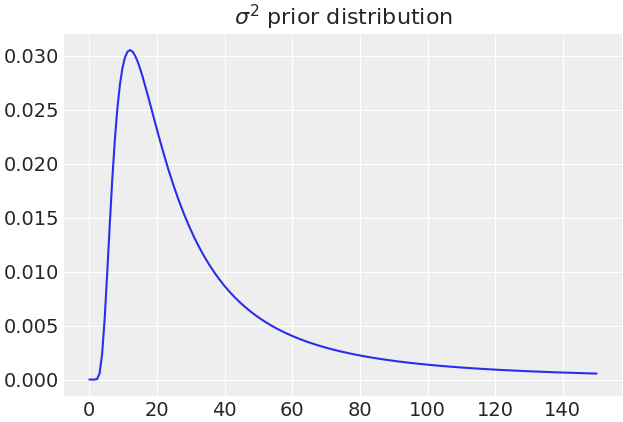
\includegraphics[scale=0.5]{../images/sigma2_prior.png}
		\caption{Função de Densidade à priori de $p(\sigma^2)$}
		\label{sig2prior}
	\end{figure}

	Veja abaixo a codificação dos hyperparâmetros à priori:
	
	\begin{lstlisting}[language=iPython]
# Prior parameters
v0 = 3
s02 = 20
a0 = v0/2
b0 = v0*s02/2
mu0 = np.zeros(3)
Lambda0 = 0.01*np.eye(3)
	\end{lstlisting}
	
	A atualização dos parâmetros conjugados é regida pelas fórmulas em \ref{posteriorformulas}. Abaixo segue o código de um função em python que recebe os parâmetros à priori $(a_0,b_0,\bd\mu_0,\bd\Lambda_0)$. O operador @ representa multiplicação matricial na sintaxe NumPy. Perceba que as fórmulas de $\hat\beta$ em \ref{betafreq}, e a fórmula de $\bd\mu_n$ envolvem o cálcul ode matriz inversa, porém por questões de eficiência, não calculamos essa inversa diretamente. Ao invés disso, é feita a resolução de um sistema linear equivalente.
	
	\begin{lstlisting}[language=iPython]
def update_parameters(X,y,a0,b0,mu0,Lambda0):
	beta_hat = np.linalg.solve(X.T@X,X.T@y)
	mu_n = np.linalg.solve(X.T@X+Lambda0,X.T@X@beta_hat+Lambda0@mu0)
	Lambda_n = X.T@X+Lambda0
	a_n = a0+n/2
	b_n = b0 + (y.T@y-mu_n.T@Lambda_n@mu_n+mu0.T@Lambda0@mu0)/2
	return dict(a_n=a_n,
		    b_n=b_n,
		    mu_n=mu_n,
		    Lambda_n=Lambda_n)
	\end{lstlisting}
	
	Executando o código acima com as prioris definidas anteriormente, obtemos os seguintes parâmetros à posteriori:
	
	\begin{align*}
		a_n&=176.5\\
		b_n&\approx733.08\\
		\bd\mu_n&\approx [-1.2762,  2.5898,  6.4903]^T\\
		\bd\Lambda_n&\approx \begin{bmatrix}
			350.01& 175  & 171.882\\
			175 &  116.8438 &  84.4265\\
			171.882 &  84.4265& 113.7668
		\end{bmatrix}
	\end{align*}

	Perceba que a média à posteriori $\bd\mu_n$ de $\beta$ é muito próxima dos estimadores de máxima verossimilhança encontrados anteriormente. Veja também que os valores da matriz de precisão estão bem alto em contraste com a precisão imprópria $\bd\Lambda_0$. 
	
	Para interpretar os parâmetros de $(a_n,b_n)$ de forma mais clara, vejamos na Figura (\ref{sig2post}) um plot da densidade da distribuição $p(\sigma^2|\bd y,\bd X)\sim\op{Inv-Gamma}(a_n,b_n)$.
	
	\begin{figure}[!htb]
		\centering
		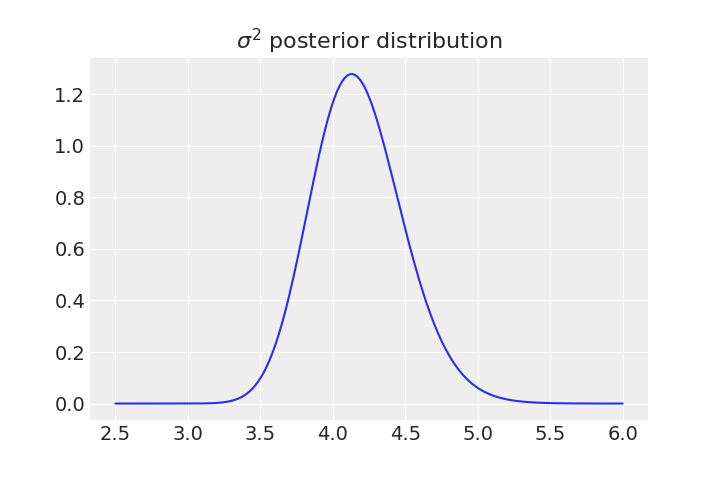
\includegraphics[scale=0.7]{../images/sigma2_posterior.png}
		\caption{Função de Densidade à posteriori de $p(\sigma^2|\bd y,\bd X)$}
		\label{sig2post}
	\end{figure}

	Perceba que mesmo com uma priori bem dispersa, a distribuição posterior está muito melhor definida, e sua média aproxima $4$ que é o seu valor real.
	
	O processo de geração de amostras à posteriori é muito simples. No caso de $\sigma^2$, geramos variáveis aleatórias $\op{Inv-Gamma}(a_n,b_n)$, utilizando o pacote SciPy. Para amostrar da distribuição condicional de $\beta$, primeiro geramos um $\sigma^2$ pela Gama-Inversa, e depois utilizando o $\sigma^2$ gerado para amostrar da distribuição $\norm(\bd\mu_n,\sigma^2\bd\Lambda_n^{-1})$.
	
	Segue abaixo o código:
	
	\begin{lstlisting}[language=iPython]
def posterior_invgamma(a_n,b_n,size=200):
  return invgamma.rvs(a=a_n, scale=b_n,size=size)
def posterior_normal(mu_n,Lambda_n,sigma2):
  sample = []
  cov = np.linalg.inv(Lambda_n)
  for s2 in sigma2:
  sample.append(multivariate_normal.rvs(mean=mu_n,cov=s2*cov))
  return np.array(sample)
posterior = update_parameters(X,y,a0,b0,mu0,Lambda0)
a_n,b_n,mu_n,Lambda_n = posterior.values()
sigma2 = posterior_invgamma(a_n,b_n,size=5000)
beta = posterior_normal(mu_n,Lambda_n,sigma2)
	\end{lstlisting}

	Como podemos ver no código geramos uma amostra de 5mil pontos. Pelos valores dos parâmetros $\bd\mu_n$ e a densidade de $\sigma^2$ à posteriri, vimos que o processo aproximou bem os valores reais dos parâmetros.
	
	Na Figura \ref{postplot} vemos a distribuição desses parâmetros.
	
	\begin{figure}[!htb]
		\centering
		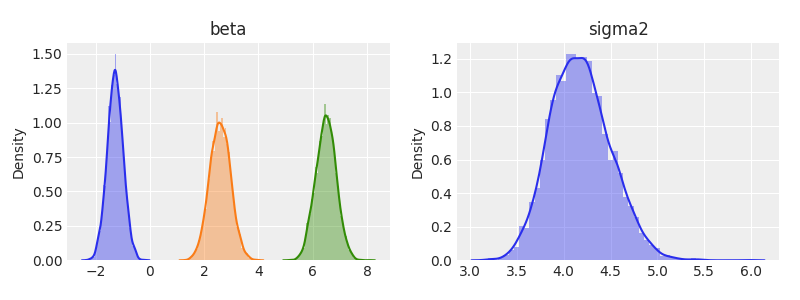
\includegraphics[scale=0.80]{../images/posterior_sampling.png}
		\caption{Legenda da figura esquerda: $\beta_0$ - Azul; $\beta_1$-Lanranja; $\beta_2$-Verde}
		\label{postplot}
	\end{figure}
	\subsection{Estimação Bayesiana - MCMC}
	
	Utilizando MCMC podemos amostrar numericamente uma distribuição à posteriori para os parâmetros. 
	
	Para $\bd\mu_0$ e $\bd\Lambda_0$ da densidade (\ref{priorbs}) de $\beta|\sigma^2$, utilizamos $\bd\mu_0=[0,0,0]^T$ e $\bd\Lambda_0=0.01\bd I$ indicando baixa precisão sobre a média nula dada à priori.
	
	Segue a codificação no PyMC3 utilizando amostrador NUTS, que é o padrão do programa. utilizamos 4 cadeias, com 5000 iterações e 1000 iterações \textit{tuning}.
	
	\begin{lstlisting}[language=iPython]
# MCMC estimation
with Model() as model:  
	# Priors
	sigma2 = InverseGamma("sigma2",alpha=a0,beta=b0)
	beta = MvNormal("beta",mu=mu0,cov=sigma2*pm.math.matrix_inverse(Lambda0),shape=(3))
	# Likelihood
	likelihood = Normal("y", mu=beta[0] + beta[1] * X1 + beta[2]*X2, sigma=sigma2**(1/2), observed=y)
	trace = sample(5000, cores=4,tune=1000)  # NUTS sampler
	\end{lstlisting}
	
	Segue na Figura (\ref{traceplot1}) 
	o gráfico do traço das cadeias e na Figura (\ref{post1})
	a distribuição à posteriori dos parâmetros gerada pela biblioteca visualição ArviZ\cite{arviz_2019}.            	
	\begin{figure}[!htb]
		\centering
		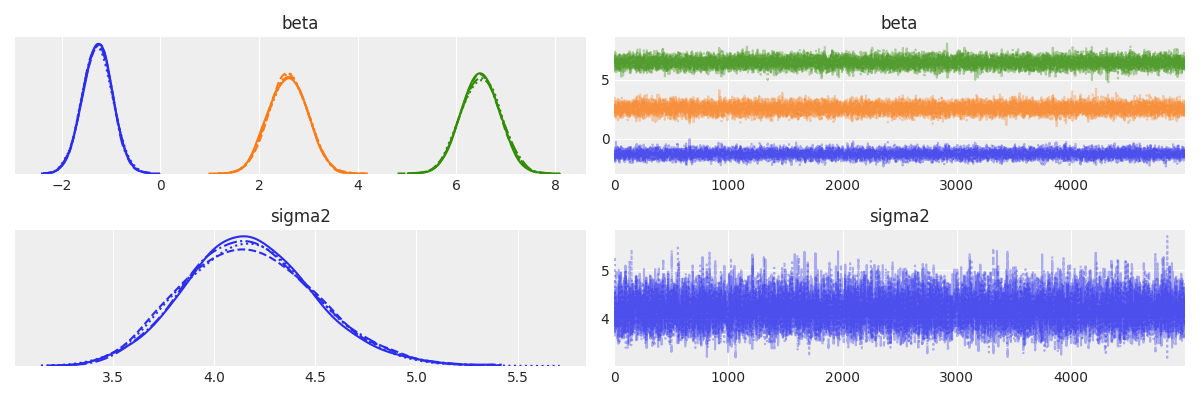
\includegraphics[scale=0.6]{../images/traceplot1.png}
		
		\caption{Plot das Cadeias de Markov}
		\label{traceplot1}
	\end{figure}
	
	\begin{figure}[!htb]
		\centering
		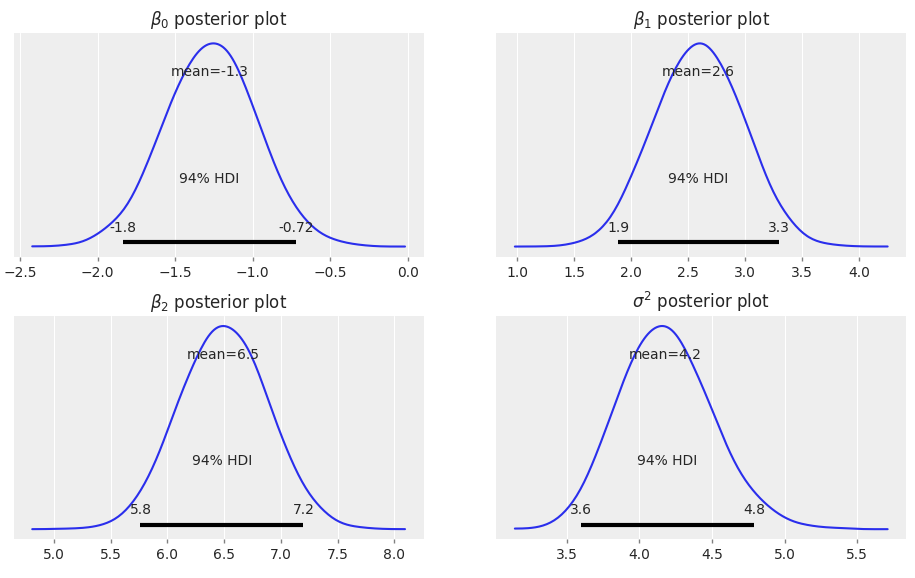
\includegraphics[scale=0.5]{../images/posteriori1.png}
		
		\caption{Distribuição à posteriori dos parâmetros}
		\label{post1}
	\end{figure}
	Visualmente podemos ver que a moda de $\sigma^2$ está próxima de $4$, $\beta_0$ (verde) próxima de -1, $\beta_1$ (laranja) perto de 3, e a moda de $\beta_2$ (verde) próxima de 6. Vemos então que as distribuições aproximaram bem os parâmetros reais. Segue abaixo as estatísticas das cadias de Markov geradas:
	
%	\begin{tabular}{lrrrrrrrr}
%		\toprule
%		{} &  mean &    sd &  hdi\_3\% &  hdi\_97\% &   ess\_sd &  ess\_bulk &  ess\_tail &  r\_hat \\
%		\midrule
%		beta[0] & -0.85 &  0.29 &   -1.40 &    -0.32 &   7296.0 &    7550.0 &    9414.0 &    1.0 \\
%		beta[1] &  2.54 &  0.38 &    1.84 &     3.25 &  10082.0 &   10085.0 &   12112.0 &    1.0 \\
%		beta[2] &  6.09 &  0.37 &    5.41 &     6.78 &  10247.0 &   10265.0 &   11648.0 &    1.0 \\
%		sigma2  &  4.06 &  0.32 &    3.48 &     4.66 &  13873.0 &   14076.0 &   11705.0 &    1.0 \\
%		\bottomrule
%	\end{tabular}
\begin{tabular}{lrrrrrrrr}
%	\centering
	\toprule
	{} &  mean &    sd &  hdi\_3\% &  hdi\_97\% &   ess\_sd &  ess\_bulk &  ess\_tail &  r\_hat \\
	\midrule
	beta[0] & -1.28 &  0.30 &   -1.84 &    -0.72 &   8569.0 &    8590.0 &   10503.0 &    1.0 \\
	beta[1] &  2.59 &  0.38 &    1.88 &     3.30 &   9832.0 &    9841.0 &   11369.0 &    1.0 \\
	beta[2] &  6.49 &  0.38 &    5.76 &     7.20 &  10736.0 &   10729.0 &   11958.0 &    1.0 \\
	sigma2  &  4.18 &  0.32 &    3.60 &     4.79 &  14823.0 &   15045.0 &   12363.0 &    1.0 \\
	\bottomrule
\end{tabular}
	
	Podemos ver que as médias à posteriori se aproximam bastante dos os estimadores frequentistas de $\beta$ e também dos parâmetros encontrados analiticamente. A primeira vantagem do modelo bayesiano é que agora temos informação sobre $\sigma^2$, que não era modelado anteriormente. Acima vemos que sua média fica próxima de $4$ com um HDI $95\%$ de $[3.48,4.66]$. Um segunda vantagem dessa modelagem, é que com uma distribuição à posteriori podemos responder perguntas como $\mathbb{P}(\beta_i\in I|\bd y,\bd X)$ para algum intervalo qualquer $I$. 
	
	Uma outra análise diagnóstica interessante a ser feita, é através dos plots de autocorrelação, na Figura (\ref{autocorr1}).
	
	\begin{figure}[!htb]
		\centering
		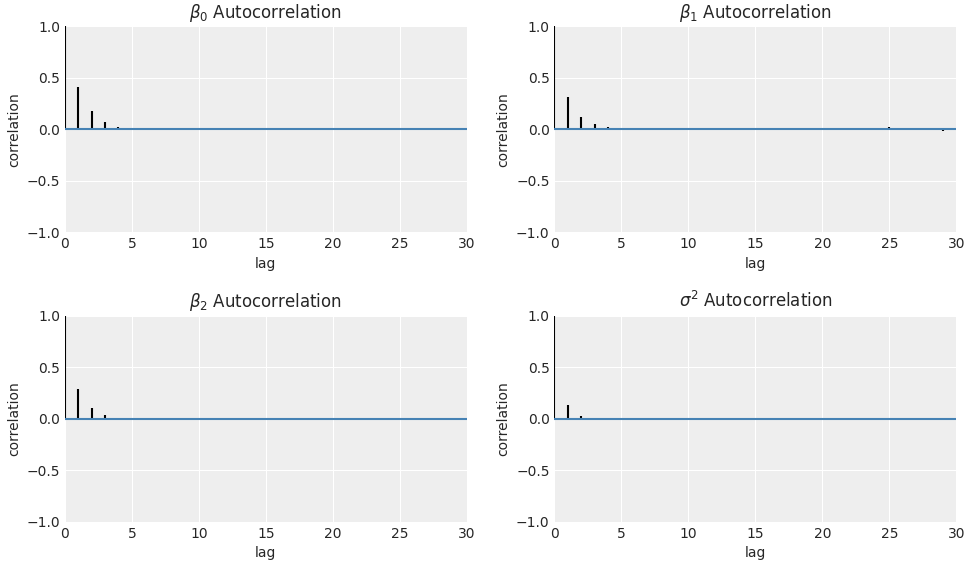
\includegraphics[scale=0.5]{../images/autocorrelation1.png}
		
		\caption{Plot de Autocorrelação}
		\label{autocorr1}
	\end{figure}

	Vemos que após poucos lags, a autocorrelação de todos os parâmetros vai pra zero, o que indica que as cadeias conseguiram convergir relativamente rápido, pois se tivéssesmos auta correlação por muitos lags, isso indicaria que o amostrador não fez uma visita satisfatória ao espaço de parâmetros, ficando ``preso'' em valores autocorrelatos.
	
	
	\newpage
	\addcontentsline{toc}{section}{Referências}
%		\bibliography{refs}
	\printbibliography
\end{document}